\chapter{Propuesta} % Main chapter title
\label{Capitulo3} % Change X to a consecutive number; for referencing this chapter elsewhere, use \ref{ChapterX}
\lhead{\emph{Propuesta}}

%----------------------------------------------------------------------------------------
%	SECTION 1
%----------------------------------------------------------------------------------------
%algorithm uses Daubechies wavelet for spatial dimension and Fourier transform for vertical dimension. 
\section{3.1 Proceso}
La propuesta consta de la combinación en cadena de los siguientes puntos:
\begin{itemize}
\item Daubichies.
\item Slices.
\item Mosaic-Malvar.
\item Blur-Shparpender.
\end{itemize}

Donde cada uno de dichas combinaciones será probada por la calidad percibida mediante el ojo humano. 
Para poder analizar las imágenes se establecieron rutas de resultados que se muestran en la Figura \ref{pics:squeme}, donde se utilizaron diversas combinaciones de la teoría mostrada en los capítulos anteriores.
\clearpage
\begin{figure}[h]
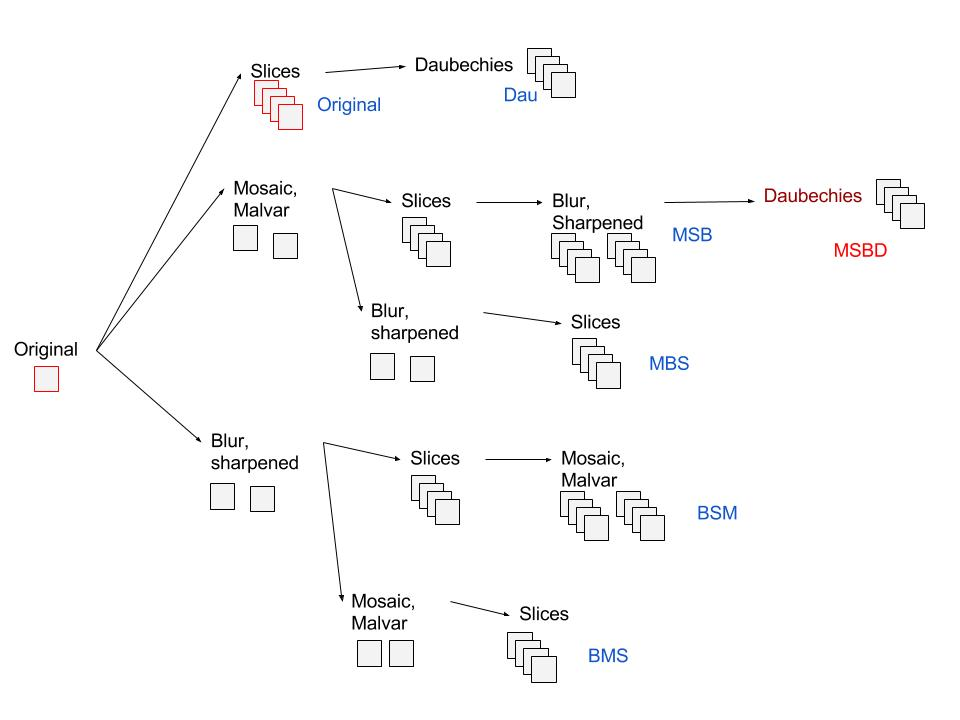
\includegraphics[scale=.4]{./images/RESULTS/squeme.jpg}
\caption{Esquema de resultados.}
\label{pics:squeme}
\end{figure}
Cada cuadro corresponde a una imagen superposicionadas y el conjunto de imágenes a las obtenidas por el procedimiento de abstracción por longitud de onda electromagnética de la imagen suporposicionada. 